\section{Systemdefinition}
\label{sec:systemdefinition}

%INTRODUKTION
%introduktion til batoff-model
Vi har fået et større indblik i, hvad problemet består af. Inden vi bevæger os videre til udarbejdelsen af systemdefinitioner (en kortfattet beskrivelse af et system udtrykt i naturligt sprog), så har vi udviklet rige billeder, der kan ses på \figref{fig:rigbillede1}, som har til formål at skabe et overblik over selve problemet. 

\begin{figure}
\centering
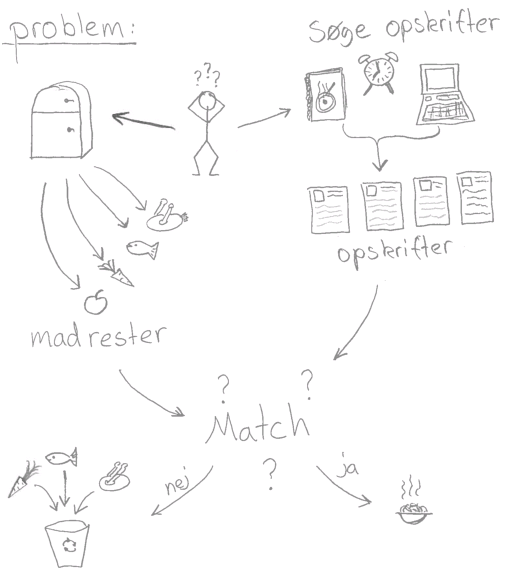
\includegraphics[scale=0.6]{billeder/rigebilleder/problemomraade.png}
\capt{Rigt billede, der visualiserer problemet ved at skulle genbruge madrester.}
\label{fig:rigbillede1}
\end{figure}

Det rige billede i \figref{fig:rigbillede1} viser en bruger, der ikke har tid eller ressourcer til at finde ud af, hvordan madresterne, der er i køleskabet, kan blive brugt i madlavningen. Det rige billede har givet os en forståelse for problemet, som vi vil bruge til udarbejdelsen af systemdefinitioner. Systemdefinitioner blev brugt til at undersøge, hvilke funktioner et system skal tilbyde, hvor det skal bruges og hvilke udviklingskriterier, der skulle gælde. Hertil benytter vi os af seks kriterier, der forkortes til BATOFF. \cite[s.~37]{ooad} BATOFF indeholdholder følgende punkter: 

\begin{itemize}[noitemsep]
\item \textbf{B}etingelser \textit{- betingelser for systemets udvikling og brug}
\item \textbf{A}nvendelsesområde \textit{- de organisationsdele, der administrerer/overvåger/styrer et problemområde}
\item \textbf{T}eknologier \textit{- den teknologi, som systemet udvikles til og ved hjælp af}
\item \textbf{O}bjekter \textit{- de væsentligste objekter i et problemområde}
\item \textbf{F}unktioner \textit{- de systemdefinitioner, som understøtter arbejdsopgaver i anvendelses området}
\item \textbf{F}ilosofi \textit{- den filosofi, der ligger bag IT-systemets anvendelse}
\end{itemize}

Disse kriterier har til formål at støtte udviklingen af systemdefinitioner ved at vurdere de forhold, der er gældende for et givet systems funktion i forhold til en organisation eller forbruger og omverden. Derudover benytter vi BATOFF-kriterierne, fordi de fastsætter nogle rammer i forhold til opsætningen og indholdet af systemdefinitioner samt opretter en form for standard, der gør det muligt at sammenligne flere forskellige systemdefinitioner på en logisk måde.

\subsection{Alternative systemdefinitioner}
\label{subsec:alternativesystemdefinitioner}

%SYSTEMDEFINITION
Vi startede med at definere selve systemdefinitionerne og derefter sikre os, at systemdefinitionerne stemmer overens med BATOFF-kriterierne. Når definitionerne var blevet udarbejdet og kontrolleret, så blev de præsenteret for informanterne.

Efter møder med vores informanter fik vi forståelsen af, at madspild er et reelt problem for de to familier. Det er blevet forklaret, hvad der ofte er grunden til madspildet, og på baggrund af møderne og det rige billede, som blev præsenteret i \secref{sec:situation} i \figref{fig:rigbillede1}, er to systemdefinitioner blevet udarbejdet.

\begin{description}
\item[Systemdefinition 1 (S1)] \hfill \\
Systemet skal fungere som et online opskriftsregister, der giver brugeren idéer til opskrifter, som kan laves ud fra de madvarer brugeren har. Systemet fokuserer på at mindske madspild, da forbrugere smider mad ud på grund af et manglende formål med anvendelsen af resterne. Brugerne af systemet er en del af en husholdning og vil have meget varierende erfaringer inden for brug af internettet. Udviklerne af systemet er ulønnede studerende. Deadline for det færdige system kan ikke ændres. Systemet skal køre på en server, der kan tilgås via en webapplikation fra en internetbrowser på enhver type computer. På baggrund af en mængde fødevarer som input, findes forskellige opskrifter, der bedst muligt matcher disse fødevarer. Opskrifterne skal kunne sorteres på flere måder, og ingredienser skal kunne tilføjes til en indkøbsliste. Ligeledes skal man kunne gemme favoritopskrifter til senere brug.
\item[Systemdefinition 2 (S2)] \hfill \\
Systemet skal fungere som et planlægningsværktøj, som har til formål at planlægge madlavningen over en given tidsperiode (\fx dage, uger, måneder) ud fra de opskrifter, der er blevet lavet over de sidste par dage. Formålet med planlægningsværktøjet er at sikre, at brugeren får en sund og varieret kost igennem udvalgte opskrifter, hvor der også tages højde for ingrediensers vitaminindhold. Brugerne af programmet vil være husstande, der har varierende erfaringer inden for brug af internettet. Udviklerne af systemet er ulønnede studerende. Systemet skal køre på en server, der kan tilgåes via en webapplikation fra en internetbrowser på enhver type computer.
\end{description}

Efter udarbejdelsen af systemdefinitionerne undersøgte vi, om de overholdte BATOFF-kriterierne. Vi havde indbyrdes i gruppen diskuteret, hvorvidt systemdefinitionerne stemmer overens med BATOFF-kriterierne. Vi har indsat de forskellige kriterier ind i \tableref{table:batoff}, hvor vi har indtastet de relevante forklaringer for de seks kriterier. 
Tabellen giver derudover et bedre overblik over systemdefinitionerne.

\ourtable{batoff}{2}{Tabel med forklaringer over BATOFF-kriterier for systemdefinitionerne S1 og S2.}
                                                 {Systemdefinitioner}
       {Kriterier        }{ Online opskriftsregister (S1) & Madplanlægger (S2)                   }{
\ourrow{Betingelser      }{ Ulønnede udviklere.           & Ulønnede udviklere.                  }
\ourrow{Avendelsesområde }{ Dele af husholdninger,        & Dele af husholdninger,               }
\ourrow{                 }{ \fx forældre eller lignende.  & \fx forældre eller lignende.         }
\ourrow{Teknologier      }{ Internetforbindelse.          & Internetforbindelse.                 }
\ourrow{                 }{ PC. Tablet. Mobiltelefon.     & PC. Tablet. Mobiltelefon.            }
\ourrow{Objekter         }{ Opskrifter. Ingredienser.     & Opskrifter. Ingredienser. Vitaminer. }
\ourrow{Funktioner       }{ Søgningsværktøj. Find         & Planlægningsværktøj. Planlægge       }
\ourrow{                 }{ opskrifter indeholdende       & madlavning ud fra                    }
\ourrow{                 }{ valgte ingredienser           & tidligere dages retter.              }
\ourrow{Filosofi         }{ Folk smider mad ud, fordi de  & Folk spiser ikke varieret nok,       }
\ourrow{                 }{ mangler et sted at            & hvilket er en trussel                }
\ourrow{                 }{ bruge deres rester.           & mod folkesundheden.                  }
}


\subsection{Valg af systemdefinition}
\label{subsec:valgafsystemdefinition}

%SYSTEMVALG
I fællesskab med informanterne, valgte vi hvilken systemdefinition, der blev valgt. Denne beslutning satte nogle fastere rammer for projektets videre forløb. Vi ønskede at høre om informanterne ville være i stand til bruge lignende systemer. Vi holdte os meget åbne for nye løsningsforslag, da vi gerne ville gøre det muligt for informanterne at komme med nye idéer, også selvom de var markant anderledes end vores systemdefinitioner. Derfor foregik møderne som semistrukturerede interviews. Det var vigtigt for os at få informanternes idéer til hvilke funktioner et sådan system skulle have og hvilke krav, de stiller.

Der blev taget højde for informanternes respons (Al dokumentation og alle referater fra de afholdte møder med informanterne kan findes i \apref{ap:informant}.) på de udarbejdede systemdefinitioner, og der blev truffet et valg, som alle parter kan se som en mulig løsning på problemerne mht. madlavning og madspild i danske husstande. Efter møderne var det helt klart, at informanterne så det online opskriftsregister (S1), der kan ses i \secref{subsec:alternativesystemdefinitioner}, som et meget brugbart system. Det mente simpelthen ikke, at et planlægningsværktøj var noget, de ville komme til at bruge. De var meget mere interesserede i at have et værktøj, der gjorde det muligt for dem at slå madrester op i et system, der ville være i stand til at give opskriter, der indeholder de indtastede ingredienser.

%AFSLUTNING
Systemdefinitionen er blevet valgt. Det er nu på tide at overveje, hvordan systemet skal fungere, hvordan det skal designes, og hvilke funktioner, der skal inkluderes i systemet.

